% !TEX root = ../main.tex

%----------------------------------------
%   SECTION TITLE
%----------------------------------------
\chapter{Two Approaches}
\label{chap:section_one}

%----------------------------------------
%   SECTION CONTENT
Most modern web applications utilize some sort of frameworks to tame the complexity of distributed computing and provide other benefits. Any complex modern web application consists of essentially 3 parts: frontend, backend, and database. These interconnected parts work together to deliver functionality to the users. The front end of a web application is the part users interact with directly via a client in a web browser. The backend handles the logic and processes that occur on the server side. It manages requests from the frontend, processes data, interacts with databases, and performs computation or business logic. Databases are where the web applications store data. They are responsible for managing the structured data that the application needs to persist.

Numerous frameworks are available today to build such web applications. Each framework provides a similar set of functionalities and comes with advantages and disadvantages. They differ in various aspects and one  important aspect is Developer Experience or DevX\cite{swimm}. Developer Experience can play a crucial role in adoption of a technology. Several key elements that directly contribute to DevX include documentation, tooling, support, and community. Bad DevX can hinder the adoption of a technology or a new framework despite its advantages, and hence it becomes an important consideration while choosing a technology or stack.

Several frameworks available today to create web applications pay enormous attention to DevX while providing features and functionality. Commonly used industry-grade frameworks include\cite{stackoverflow}:

\begin{itemize}
    \item Frontend frameworks: Angular, React\cite{react} and VueJs
    \item Backend frameworks: Node.js, Express\cite{express}, ASP.NET core
    \item Databases: PostgreSQL, MySQL, SQLite, MongoDB
\end{itemize}

\section{First Approach: TEASync}
\label{section:first_approach}

TEASync acts as a real-time collaboration platform built using Haskell,
and in which developers develop in a single Elm-language project. In the high-level design of the system, it manages the WebSocket connections and communication between clients and servers.

TEASync can be used to develop multi-player applications using a single programming language,
in a single project, with ``local'' and ``global'' aspects in the same modules.
Figure~\ref{fig:teasync-architecture} shows two local (client) interactions with green background (top and bottom),
and global interactions with orange background in the middle.
The local interactions follow exactly the same pattern as the Elm architecture (TEA) (Model-View-Update) used by Elm developers.
The additional global layer and interconnections follow as closely as possible the conventions and vocabulary used to describe TEA.
The main advantage of using a framework such as TEASync is that developers do not need to learn different technology stacks and programming languages to build multi-client applications. This is highly beneficial, especially for prototyping when we do want to make an architectural decision about choosing a technology stack.

Using Elm, the developer can define state and logic for a multi-client application without the need to worry about underlying communication infrastructure. Using the SDDraw tool, developers can define application states and incorporate them to enhance DevX. A backend server using WebSockets\cite{websockets} will sync messages across multiple clients, with virtual servers  spawned in the development environment STaBL.Rocks.


\begin{figure}[ht]
    \centering
    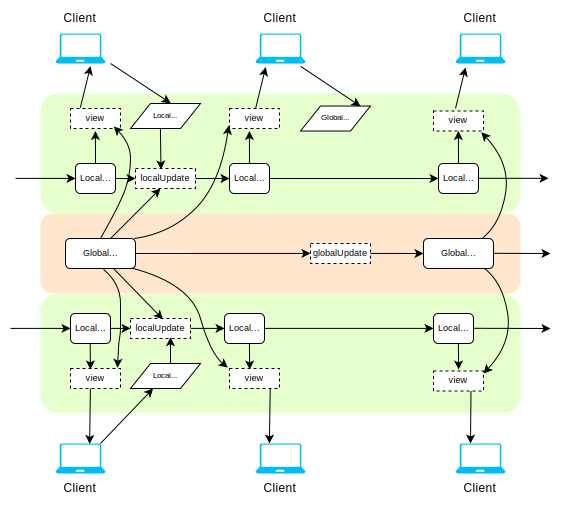
\includegraphics[width=0.8\textwidth]{diagrams/TEASyncAppArchitecture.png}
    \caption{TEASync Architecture}
    \label{fig:teasync-architecture}
\end{figure}

\section{Second Approach: React, NodeJs, Express, and other libraries}
\label{section:second_approach}

React is a very popular front-end development framework for building complex web applications. NodeJs\cite{nodejs} serves as backend environment running backend services making it possible to sync data and messages across the different clients. Other libraries are used to reduce the boilerplate code and fill in the functionalities a certain framework lacks.

\subsection{Why React?}
We made the following considerations when choosing React as the front-end framework:

\begin{itemize}
    \item Support for programming in both JavaScript and TypeScript languages.
    \item Support for reusable components, saving time and effort.
    \item Existence of a wide range of packages and libraries.
    \item Strong community of developers who contribute to it and provide support.
\end{itemize}

\textbf{Programming Language support}

Developers can write React components using JavaScript and TypeScript languages. This option allows the developer to choose between the two popular choices for building web applications. JavaScript is more versatile, as many other front-end and back-end frameworks use JavaScript. 

\textbf{Reusable components}

React lets developers define components of the application and reuse them in different parts of the application. This reduces the time and efforts of the developer while building a large complex application. Reusable components increase uniformity and aid in effective testing of the application.

\textbf{Packages and Libraries}

React supports thousands of packages and libraries to solve various problems one may encounter during the application development phase. Many libraries are inter-operable, which creates an ecosystem that allows developers to pick and choose the tools they need to build robust, scalable, and maintainable applications. This ecosystem fosters innovation, collaboration, and rapid development, enabling developers to build complex applications quickly and efficiently. With new libraries and tools constantly emerging, the React ecosystem is constantly evolving, providing developers with a wide range of solutions to tackle even the most complex challenges.

\textbf{Community support}

React’s community support is one of its strongest assets, providing a robust foundation for developers to build and maintain applications. With a massive global community of developers, React’s ecosystem is fueled by thousands of active contributors who contribute to React’s core codebase. React’s official documentation is comprehensive and well-maintained, with numerous tutorials, guides, and blog posts available to help developers learn and grow. 

\section{Applications}
\label{section:applications}

\subsection{First Application: Chatroom}


The chatroom allows a mentor to set up a chatroom and credentials required to join the chatroom. Once a mentor creates a chatroom, the users can join the session using the credentials set up by the mentor. The chatroom synchronizes messages for all connected clients.

\subsection{Second Application: Calendar-Sync}

Calendar-Sync app allows users to add and modify events on a calendar. The events will we visible to all the users along with their (editable) attributes, such as start time and end time. 

%----------------------------------------

% \blindtext[3]